%!TEX program = xelatex
%!BIB program = bibtex
\documentclass[cn,black,12pt,normal]{elegantnote}
\usepackage{float}
\usepackage{hyperref}
\usepackage{amsmath}
\usepackage{amsfonts}
\usepackage{amssymb}
\usepackage{siunitx}[=v2]
\usepackage{fancyhdr}
\usepackage{newtxtext}
\usepackage{algorithm}
\usepackage{algorithmic}
\newcommand{\uct}[1]{\textsuperscript{\textsuperscript{\cite{#1}}}}
\renewcommand{\tablename}{\textbf{Table}}
\renewcommand{\figurename}{Figure.}
\renewcommand{\refname}{References}
\renewcommand{\contentsname}{Contents}
\renewcommand{\versiontext}{Version: }
\renewcommand{\updatetext}{Update: }
\PassOptionsToPackage{no-math}{fontspec}
\lstset{basicstyle=\footnotesize\ttfamily\color[RGB]{50,0,130},numbers=none,frame=trBL}

\sisetup{mode=text}
\sisetup{range-phrase = \text{ \textasciitilde }}
\pagestyle{fancy}
\fancyhead[L]{School of Software Engineering, Tongji University}
\fancyhead[R]{Data Structure Projects}
\renewcommand{\headrulewidth}{1pt}

\title{n-Queens Puzzle\\N皇后问题}
\author{1951510\; 姜文渊}
\institute{\small \url{https://github.com/jwyjohn/Jwy_DataStructureHomework}}
\version{0.50}
\date{\today}

\begin{document}

\maketitle

\tableofcontents

\newpage

\section{Introduction}

The eight queens problem, also known as the eight queens puzzle, is the problem of placing eight chess queens on an $8 \times 8$ chessboard so that no two queens threaten each other; thus, a solution requires that no two queens share the same row, column, or diagonal. The eight queens puzzle is an example of the more general $n$ queens problem of placing $n$ non-attacking queens on an $n \times n$ chessboard, for which solutions exist for all natural numbers n with the exception of $n = 2$ and $n = 3$.\uct{wiki:Eight_queens_puzzle}

This project uses the backtracking algorithm with a stack to solve the n-Queens Puzzle. Although the more popular way of implementing backtracking algorithms is the recursive function, a stack can offer a better understanding and control of such backtracking algorithms.

\section{Demostration}

\subsection{Compile and run the program}

On linux platform with \lstinline{make} and a \lstinline{g++} which supports C++ 11 Standard, just \lstinline{cd} to the \lstinline{./linux} and run \lstinline{make build}. The binary executable will be generated in the same directory named as \lstinline{a.out} or \lstinline{queen}, according to the configurations in the \lstinline{Makefile}. Use \lstinline{./a.out} to run the program.

(On windows platforms, you may need to adjust the max stack size manually, to avoid stack overflow when n>10, since default stack size of windows tend to be much smaller.)

The program is an interactive shell, where you can input commands and get results.

\begin{figure}[H]
    \centering
    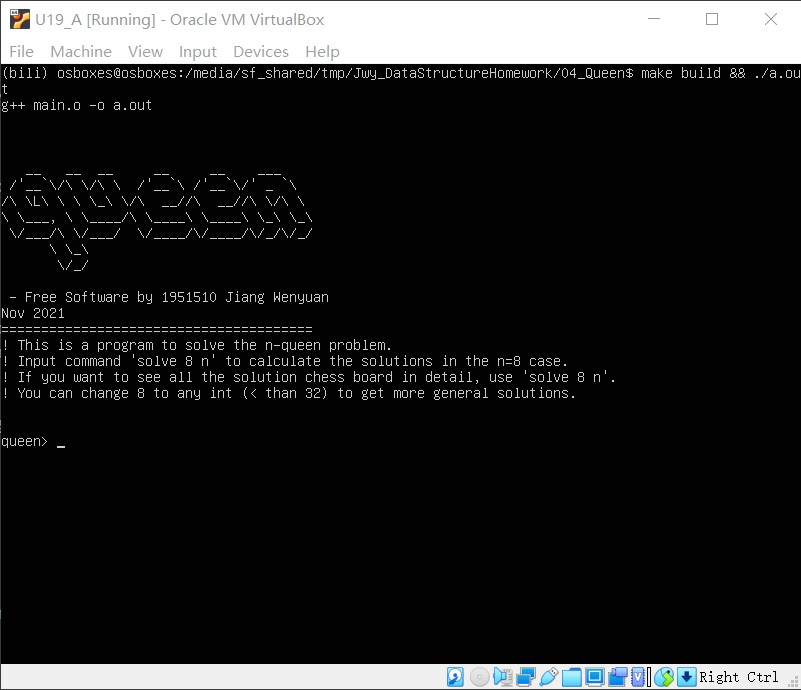
\includegraphics[width=0.7\linewidth]{image/queen_01.jpg}
    \caption{The user interface of the program}
\end{figure}

Usage of commands can be found on the main screen, and the \lstinline{help} command can give you information about theses commands.  All available commands is listed below.

\begin{enumerate}
    \item \lstinline{help} : Show help for a certain command.
    \item \lstinline{exit} : Exit the program.
    \item \lstinline{solve [N] (y/n)} : Solve the \lstinline{[N]} Queens puzzle, where \lstinline{[N]} is an integer $> 0$ and $< 25$ (the limits depend on your conf and platform). If you want to see all solution chessboards, use \lstinline{solve [N] y}, or the \lstinline{solve [N] n} will just output the number of solutions.
\end{enumerate}

\subsection{Solve a case}

Type \lstinline{solve 8 y} to solve the case where $N=8$, and print all solutions. For this case, you can get 92 solutions, with queen marked as \lstinline{X} and empty space marked as \lstinline{O}. If your terminal history buffer is too small for such results, try adjust the terminal settings.

Also, type \lstinline{solve 8 n} can give out number of solutions, but not printing all the cases, which might be useful if you do not care about specific solutions.

\begin{figure}[H]
    \centering
    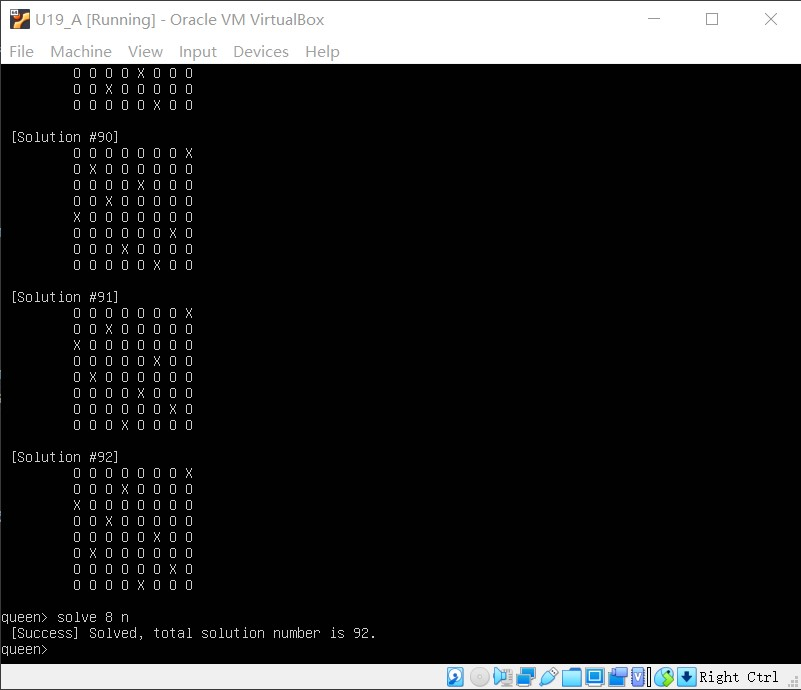
\includegraphics[width=0.7\linewidth]{image/queen_02.jpg}
    \caption{Use \lstinline{test} to run a sort}
\end{figure}

\section{Stack and backtracking}

\subsection{About the stack}

In computer science, a stack is an abstract data type that serves as a collection of elements, with two main principal operations\uct{wiki:Stack_(abstract_data_type)}:
\begin{enumerate}
    \item Push, which adds an element to the collection
    \item Pop, which removes the most recently added element that was not yet removed
\end{enumerate}

The order in which elements come off a stack gives rise to its alternative name, \textbf{LIFO (last in, first out)}. Additionally, a peek operation may give access to the top without modifying the stack (like \lstinline{s.top()} in C++).\uct{wiki:Stack_(abstract_data_type)}

A stack can be easily implemented either through an array or a linked list, and many other ways to implement a stack also exist.

\subsection{About the backtracking algorithm}

Backtracking is a general algorithm for finding solutions to some computational problems, notably constraint satisfaction problems, that incrementally builds candidates to the solutions, and abandons a candidate ("backtracks") as soon as it determines that the candidate cannot possibly be completed to a valid solution.\uct{gurari1999cis}

Backtracking can be applied only for problems which admit the concept of a "partial candidate solution" (like the eight queen puzzle here) and a relatively quick test of whether it can possibly be completed to a valid solution. It is useless, for example, for locating a given value in an unordered table. When it is applicable, however, backtracking is often much faster than brute-force enumeration of all complete candidates, \textbf{since it can eliminate many candidates with a single test}.\uct{wiki:Backtracking}

The pseudocode for a general backtracking algorithm is shown below.

\begin{algorithm}[H]
    \caption{Backtracking algorithm: \textbf{backtrack}$(c)$}
    \label{alg1}
    \begin{algorithmic}
        \IF{\textbf{REJECT}$(P,c)$}
        \STATE \textbf{RETURN}
        \ENDIF
        \IF{\textbf{ACCEPT}$(P,c)$}
        \STATE \textbf{OUTPUT}$(P,c)$
        \STATE \textbf{RETURN}
        \ENDIF
        \STATE $X \gets$ \textbf{FIRST}$(P,c)$
        \WHILE{$s \neq$ NULL}
        \STATE \textbf{backtrack}$(c)$
        \STATE $X \gets$ \textbf{NEXT}$(P,c)$
        \ENDWHILE
    \end{algorithmic}
\end{algorithm}

Where \textbf{REJECT}$(P,c)$ and \textbf{ACCEPT}$(P,c)$ judges if current solution $c$ suits the problem $P$, and \textbf{FIRST}$(P,c)$, \textbf{NEXT}$(P,c)$ gives the solutions derived from $c$.

\subsection{Use backtracking with stack}
The pseudocode above is a recursive function, therefore it can be implemented by a stack. The stack can be a system stack, which is provided by the OS and the construction of the stack is automatically done by the compiler. Or the stack can be a user-defined one, which is the case in the author's code.

The stack is used to save information of the most recently checked chessboard. All the (till-now) eligible chessboards derived from the most recently checked chessboard are pushed into the stack for further checking. If a chessboard is accepted, then it is added to the results and poped from the stack.

The pseudocode for the n-queen algorithm is shown below.
\begin{algorithm}[H]
    \caption{solve N-queen}
    \label{alg2}
    \begin{algorithmic}
        \STATE Put empty chessboard to stack.
        \WHILE{Stack not empty.}
        \STATE Get the top chessboard from the stack and POP it.
        \IF{Chessboard has N queens.}
        \STATE Save the chessboard to results.
        \ELSE
        \STATE PUSH all the eligible chessboards with one more queen to stack.
        \ENDIF
        \ENDWHILE
    \end{algorithmic}
\end{algorithm}

\section{Notes on the source code}

In the author's source code \lstinline{main_header.h}, you can find a definition of a struct \lstinline{sort_func_result} like this:
\begin{lstlisting}[language = C++]
struct chessboard
{
	int current_queen_num = 0;
	int board[MAX_CHESSBOARD_SIZE][MAX_CHESSBOARD_SIZE];
};
\end{lstlisting}
This struct is used for store the unfinised chessboards in the backtracking process, where \lstinline{current_queen_num} is the number of queens that have already been on the chess board without threatening each other, and the 2-d array \lstinline{board[MAX_CHESSBOARD_SIZE][MAX_CHESSBOARD_SIZE]} is the chessboard data.

The function used to check if the position $(x,y)$ on a given chessboard is safe for placing another queen is \lstinline{bool is_queen_safe(chessboard a, int x, int y)}, as is shown in the code below.
\begin{lstlisting}[language = C++]
bool is_queen_safe(chessboard a, int x, int y)
{
	if (x > N || y > N)
		return false;
	int Dx[8] = {+1, -1, 0, 0, +1, -1, +1, -1};
	int Dy[8] = {0, 0, +1, -1, +1, +1, -1, -1};
	for (int k = 0; k < 8; k++)
	{
		int dx = Dx[k], dy = Dy[k];
		int i = x, j = y;
		while (0 <= i && i <= N && j >= 0 && j <= N)
		{
			flag = flag && !a.board[i][j];
			i = i + dx, j = j + dy;
		};
	};
	return flag;
};
\end{lstlisting}

Instead of using a bunch of nested \lstinline{if}s, the author uses a direction vector \lstinline{Dx,Dy} to determine the position for checking. This may cause some performance burden, but it can make the code easier to understand.

Then is the main loop for operating the stack and generate the results.

\begin{lstlisting}[language = C++]
int queen_solution(int n, bool show_board)
{
	N = n;
	chessboard a;
	stack<chessboard> s, ans;
	s.push(a);
	while (!s.empty())
	{
		chessboard tmp = s.top();
		s.pop();
		tmp.current_queen_num++;
		int i = tmp.current_queen_num;
		for (int j = 1; j < N + 1; j++)
		{
			if (is_queen_safe(tmp, i, j))
			{
				tmp.board[i][j] = _QUEEN;
				if (i < N + 1)
				{
					s.push(tmp);
				}
				if (i == N)
				{
					ans.push(tmp);
				};
				tmp.board[i][j] = 0;
			};
		};
	};
....
\end{lstlisting}
As you can see in the code, the \lstinline{while (!s.empty())} is where the backtracking is done. Inside the \lstinline{while (!s.empty())} loop, a \lstinline{for (int j = 1; j < N + 1; j++)} loop is used to generate next solutions, and inside the for loop, whether to accetp a solution is determined.

The source code may help you understand how each algorithm actually works. Most of the code in \lstinline{main.cpp} is for processing the user's input, which is not so interesting.

\section{Discussion}

\subsection{The history perspective}
The eight queens problem was first raised by Chess composer Max Bezzel in 1848, and later Franz Nauck gave out the first solutions in 1850.\uct{rouse1960eight} Later, in 1972, \textbf{Edsger Dijkstra} used this problem to illustrate the power of what he called structured programming. He published a highly detailed description of a depth-first backtracking algorithm. \uct{wiki:Eight_queens_puzzle}

\subsection{The mathematics perspective}
It has been proved that the number of n-queen solutions has asymptotics of the form:
\begin{equation}
    O(n) = ((1\pm o(1))ne^{-\alpha})^n
\end{equation}
with $\alpha = 1.942 \pm 3 \times 10^{-3}$\uct{simkin2021number}.

Some of the solution numbers are listed in the table below.
\begin{table}[H]
    \caption{\textbf{Number of solutions of N queens puzzle}}
    \centering
    \begin{tabular}{c|ccccc}
        \toprule
        N         & 1   & 4   & 8    & 16          & 24                   \\
        \midrule
        Solutions & $1$ & $1$ & $92$ & $14,772,512$ & $227,514,171,973,736$ \\
        \bottomrule
    \end{tabular}
\end{table}

As can be seen in the table, the number of solutions exploded when $n$ gets bigger. In fact, the $27 \times 27$ board is the highest-order board that has been completely enumerated.
\begin{equation}
    Q(27) = 234907967154122528
\end{equation}
The result is calculated by FPGA rather than ordinary computers, and you can find the methods on GitHub here \url{https://github.com/preusser/q27}.\uct{preusser2017putting}

Thus, the computational complexity of solving n-queens problem by backtracking algorithm is far greater than $O(2^n)$, and the same is ture for the memory needed to solve this problem (which is the max stack size here).

\subsection{More than just queens}

If we modify the function \lstinline{bool is_queen_safe(chessboard a, int x, int y)}, we can solve problems like n-knight, n-rook, or n-bishop problems, with the same backtracking \lstinline{while (!s.empty())} loop.

In fact, 32 knights, or 14 bishops, 16 kings or 8 rooks, can be put on one $8 \times 8$ chessboard "Peacefully" without threatening each other. Detailed solutions is found using the backtracking method.

\bibliography{references}
\end{document}
